\documentclass{practice}

\usepackage{pgfplots}
\pgfplotsset{width=20cm,compat=1.18}
\usepgfplotslibrary{external,fillbetween}

\usepackage[dvipsnames,hyperref]{xcolor}

\begin{document}
\begin{center}
  \textbf{Practice 5, solutions}
\end{center}

\begin{task}{Function growth}
  % https://ggc-discrete-math.github.io/growth_functions.html
  Ordering of basic functions by growth:
  \begin{multline*}
    \Oh(1) \le
    \Oh(\log n) \le
    \Oh\Bigl(\sqrt[\leftroot{-2}\uproot{2}3]{n}\Bigr) \le
    \Oh\Bigl(\sqrt{n}\Bigr) \le
    \Oh(n) \\\le
    \Oh\bigl(n^2\bigr) \le
    \Oh\bigl(n^3\bigr) \le
    \Oh\bigl(2^n\bigr) \le
    \Oh\bigl(3^n\bigr) \le
    \Oh(n!) \le
    \Oh\bigl(n^n\bigr).
  \end{multline*}

  \iffalse
  \begin{figure}[h!]
    \centering
    \begin{tikzpicture}
      \begin{axis}[
        width=10cm,
        axis lines = left,
        grid=major,
        grid style={dashed},
        xlabel=$n$,
        ylabel=Growth,
        restrict x to domain=0:10,
        restrict y to domain=0:10,
        domain=0:10,
        xmin=0,ymin=0,
        xmax=11,ymax=11,
        samples=1000
      ]
        \addplot[thick] {log2(x)}
        node[above,pos=1]{$\Oh(\log_2(n))$};
        \addplot[thick] {pow(x,1/2)}
        node[above,pos=1]{$\Oh(\sqrt(n))$};
        \addplot[thick] {x};
        \addplot[thick] {x^2};
        \addplot[thick] {2^(x)};
        \addplot[thick] gnuplot{gamma(x+1)};
      \end{axis}
    \end{tikzpicture}
  \end{figure}
  \fi

  For the second question, because multiplying each function by $n$ preserves the order, we have
  \[
    n \log n,\quad
    n\cdot n,\quad
    n\cdot n^{1/3}
  \]
  and so, from the ordering $\Oh(\log n) \le \Oh\bigl(n^{1/3}\bigr) \le \Oh(n)$
  we deduce that
  \[
    \Oh(n\log n) \le \Oh\bigl(n^{4/3}\bigr) \le \Oh\bigl(n^2\bigr).
  \]
\end{task}

\begin{task}{Estimate the $\Oh\bigl(f(n)\bigr)$}
  \begin{itemize}
    \item $f(n) = 2n + 3n^2 + 100$
    
    Because the highest order term is $3n^2$, we deduce that $f(n) = \Oh\bigl(n^2\bigr)$, which is \emph{quadratic complexity}.
    We then require
    \[
      2n + 3n^2 + 100 \le cn^2
    \]
    and by picking $n_0=1$ and by summing up the absolute values of the polynomial coefficients, we get $c \ge 105$.
    Note that this trick works for polynomials, but not necessarily for other types of functions!

    \item $f(n) = -7n^3 - n^2 + n - 3$
    
    The highest order term is $-7n^3$ and so we have $f(n) = \Oh(n^3)$, which is \emph{cubic complexity}.
    By the same method as above, we pick $n_0=1$ and we thus get $c \ge 12$.

    \item $f(n) = \log(n) + 5n$
    
    The highest order term is $5n$ and so we have $f(n) = \Oh(n)$, which is \emph{linear complexity}.
    Recall that $\log(n) < n$ for all $n > 0$.
    We then have
    \[
      \log(n) < n
      \qquad\iff\qquad
      \log(n) + 5n < n + 5n = n(1 + 5)
    \]
    for $n>0$ and by picking $n_0 = 1$ we have $c \ge 6$.

    \iffalse
    \item $f(n) = 11n + 2^n + 0.2n^3$
    
    This is tricky, because we do not have a good way to solve the inequality:
    \[
      11n + 2^n + 0.2n^3 \le c2^n
    \]
    due to it being a mix of exponentials and polynomials.
    Let us fix $c = 10$ and compute the first and second derivatives of $h(n)=f(n)/(10g(n))$.

    We have
    \begin{align*}
      h'(n) &= \frac{10g(n)f'(n) - 10f(n)g'(n)}{(10g(n))^2}\\
      &=
    \end{align*}
    \fi
    
    \iffalse
    Note that we can write $f(n) = n\bigl(11 + 0.2n^2\bigr) + 2^n$.
    Fixing $c = 10$ gives us
    \begin{align*}
      n\bigl(11 + 0.2n^2\bigr) + 2^n &\le 10 \cdot 2^n\\
      n\bigl(11 + 0.2n^2\bigr) &\le 9\cdot 2^n
    \end{align*}
    which is a bit trickier to solve than polynomial inequalities.

    Because both sides of the inequality are positive for $n \ge 1$, we can take the logarithm on both sides.
    We have
    \begin{align*}
      \log\bigl(n\bigl(11 + 0.2n^2\bigr)\bigr) &\le \log(9\cdot2^n)\\
      \log(n) + \log\bigl(11+0.2n^2\bigr) &\le \log(9) + \log\bigl(2^n\bigr)\\
      \log(n) + \log\bigl(11+0.2n^2\bigr) &\le \log(9) + n\\
      2^{\log(n) + \log\bigl(11+0.2n^2\bigr)} &\le 2^{\log(9) + n}\\
    \end{align*}

    Recall that
    \[
      \log_b(b^x) = x
    \]
    \fi

    \item $f(n) = 10 + 2^n + 2n^2$
    
    The highest order term is $2^n$ and so $f(n) = \Oh\bigl(2^n\bigr)$, which is \emph{exponential complexity}.
    Since here we do not have a polynomial, we cannot use the same approach as for the previous approaches.
    Instead, let us fix $n_0$ and compute the maximum value that $h(n)=f(n)/g(n)$ can take.
    Then, we fix $c \ge \max(f(n)/g(n))$ in the range $[n_0, \infty)$.

    Let us observe the behaviour of $h(n)$ by computing its first derivative.
    We have
    \begin{align*}
      h'(n) &= \frac{g(n)f'(n)-f(n)g'(n)}{\bigl(g(n)\bigr)^2}\\
      &= \frac{
        2^n(4n + 2^n\ln2) -
        (10 + 2n^2 + 2^n)2^n\ln2
        }{2^{2n}}\\
      &= \frac{4n + 2^n\ln(2) - 10\ln(2) - 2n^2\ln(2) - 2^n\ln(2)}{2^n}\\
      &= \frac{-2\ln(2)n^2 +4n - 10\ln2}{2^n}\\
      &= -\frac{\ln(2)n^2 - 2n + 5\ln2}{2^{n-1}}
    \end{align*}
    which is clearly negative when $\ln(2)n^2 -2n + 5\ln(2)>0$.
    Because the leading coefficient $\ln(2)>0$, the parabola opens upwards and so the function is positive for values of $n$ larger than its largest root, or always positive if it has no real roots.

    We have $\Delta = (-2)^2 - 4 \cdot \ln{2} \cdot 5\ln{2} = 4 - 20\ln^2(2) \le 0$ and so the function does not have any real roots.
    In turn, this implies that $h'(n)$ negative for all values of $n$, meaning that $h(n)$ is monotonically (strictly) decreasing.
    You can visually confirm this with \autoref{fig:graph}.

    \begin{figure}[h!]
      \centering
      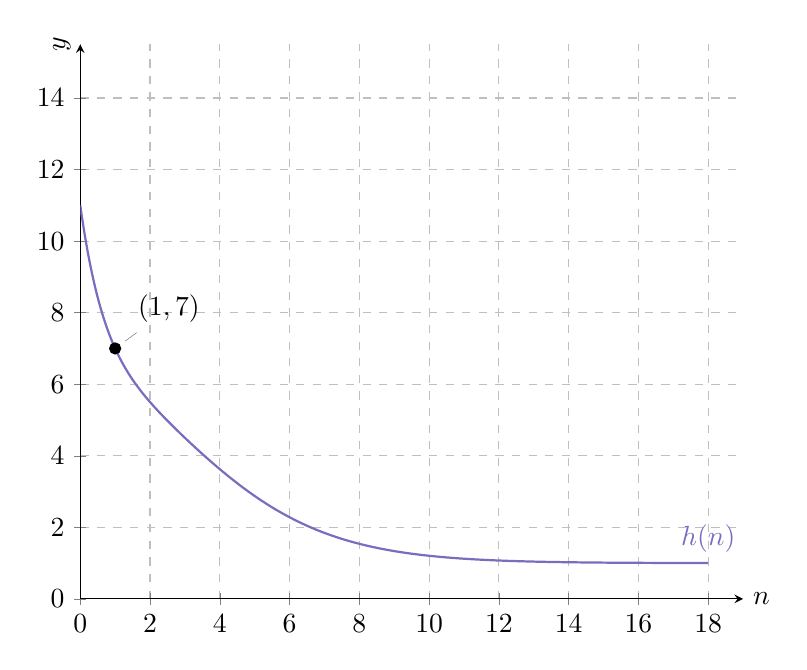
\begin{tikzpicture}
        \begin{axis}[
          width=10cm,
          axis lines = left,
          grid=major,
          grid style={dashed},
          xlabel=$n$,
          xlabel style={at=(current axis.right of origin), anchor=west},
          ylabel=$y$,
          ylabel style={at=(current axis.above origin), anchor=south},
          domain=0:18,
          xmin=0,ymin=0,
          xmax=19,ymax=15.5,
          samples=1000
        ]
          \addplot[thick,Periwinkle] {(10 + 2*pow(x, 2) + pow(2, x))/pow(2, x)}
          node[above,pos=1]{$h(n)$};;
          \addplot[mark=*] coordinates {(1,7)} node[pin={[pin distance=1mm]50:{$(1,7)$}}]{};
        \end{axis}
      \end{tikzpicture}
      \caption{Graph for $h(n)=f(n)/g(n)$.}
      \label{fig:graph}
    \end{figure}

    This means that if we pick $n_0$ and evaluate $h(n_0)$, we get the maximum of $h(n)$ in the interval $[n_0, \infty)$.
    By fixing $n_0 = 1$ we have $h(n) = (10 + 2 + 2)/2 = 7$ and so $c \ge 7$.
    You can visually confirm this with \autoref{fig:asymptote}.

    \begin{figure}[h!]
      \centering
      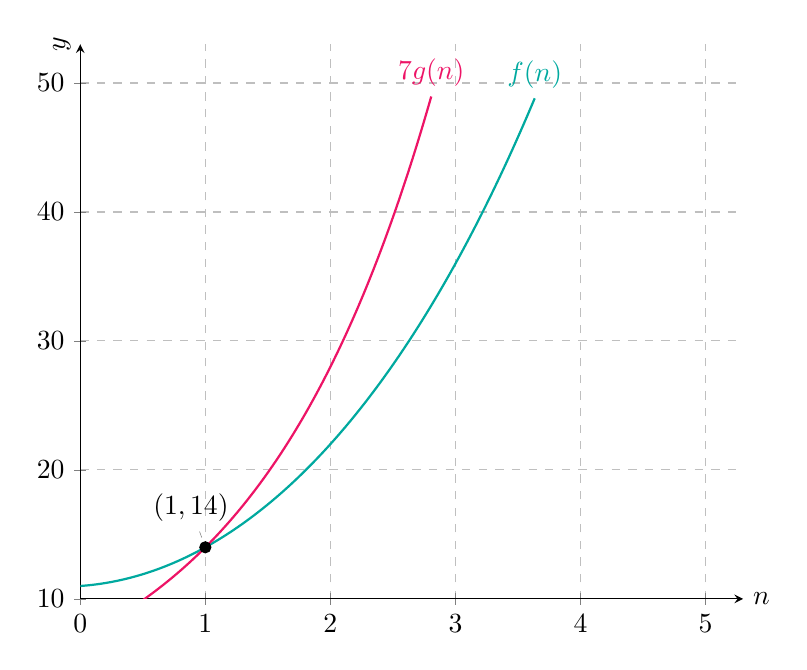
\begin{tikzpicture}
        \begin{axis}[
          width=10cm,
          axis lines = left,
          grid=major,
          grid style={dashed},
          xlabel=$n$,
          xlabel style={at=(current axis.right of origin), anchor=west},
          ylabel=$y$,
          ylabel style={at=(current axis.above origin), anchor=south},
          domain=0:30,
          restrict y to domain=9:49,
          xmin=0,ymin=10,
          xmax=5.3,ymax=53,
        ]
          \addplot[thick,Emerald,samples=1000] {10 + 2*pow(x, 2) + pow(2, x)}
          node[above,pos=1]{$f(n)$};
          \addplot[thick,WildStrawberry,samples=2000] {7*pow(2, x)}
          node[above,pos=1]{$7g(n)$};
          \addplot[mark=*] coordinates {(1,14)}
          node[pin={[pin distance=1mm,left=1em,above]50:{$(1,14)$}}]{};
        \end{axis}
      \end{tikzpicture}
      \caption{Graph of $f(n)$ and $7g(n)$.}
      \label{fig:asymptote}
    \end{figure}

    \begin{tcolorbox}[title=Derivative test]
      While we do not expect you to solve complex derivatives, you should be aware of the derivative test.
      For example, it may be that we will give you the derivative in the exam in case $f(n)/g(n)$ is a complex expression, and then you can (and might have to) rely on it to find $c$.
    \end{tcolorbox}

    \iffalse
    Now we must check whether $h'(n)$ is negative for $n=n_0=10$.
    Since $20\ln(2) > 11$, we have that $h'(10)<0$.
    Because $h'(n)_{n>1}$ is also monotonically decreasing, it will remain negative for all values of $n > n_0$.
    This means that $h(n)$ is decreasing for all values of $n > n_0$, and that $h(n)$ takes its maximum value for $n\in[n_0, \infty)$ at $n_0$.

    We have $h(n_0) = f(10)/g(10) = (110 + 20 + 1024)/1024 = 1154/1024 \approx 1.13$.
    Thus $n_0 = 10$ and $c \ge 2$ will satisfy the definition.
    \fi

    \item $f(n) = n \log(n) + n^{1.5}$
    
    We have
    \[
      f(n) = n\log(n) + n^{1.5} = n \log(n) + n \cdot n^{1/2}
    \]
    and since we know that $\sqrt{n}$ grows faster than $\log(n)$, it follows that $f(n)=\Oh\bigl(n^{1.5}\bigr)$.

    Let us fix $n_0 = 1$, and find a $c$ which would satisfy the definition.
    To do so we can try to compute the maximum value that $h(n)=f(n)/g(n)$ can take in the interval $[n_0, \infty)$, and then fix $c \ge \max$.
    This approach is reliable, although it is not always the simplest.

    To find the maximum of $h(n)$, we compute its first derivative $h'(n)$, and observe its behaviour in the interval $[n_0, \infty)$.
    If it is monotonically decreasing, the value of $h(n_0)$ is guaranteed to be the maximum in that interval.
    If not, then we must find the critical points of the derivative, i.e. values of $n$ such that $h'(n)=0$.
    The critical points are the points after which the function's behaviour might change, e.g. from increasing to decreasing.

    Before we compute the derivative $h'(n)$, let us compute the derivative of $n\log(n)$.
    We have:
    \begin{align*}
      \bigl(n\log(n)\bigr)' &= n(\log(n))' + \log(n)\\
      &= \frac{n}{n \ln(2)} + \log(n)\\
      &= \frac{1}{\ln(2)} + \frac{\ln(2)\log(n)}{\ln(2)}\\
      &= \frac{1+\ln(n)}{\ln(2)}
    \end{align*}
    \begin{tcolorbox}[title=Log base switch]
      To get from the third line to the fourth line, I used the property:
      \[
        \log_b(a)\log_c(b) = \log_c(a).
      \]
      \tcblower
      \[
        \log(n)\ln(2) = \log_2(n) \cdot \log_e(2) = \log_e(n) = \ln(n)
      \]
    \end{tcolorbox}

    Let us compute the first derivative:
    \begin{align*}
      h'(n) = \frac{g(n)f'(n) - f(n)g'(n)}{\bigl(g(n)\bigr)^2}
      &= \frac{
        n^{1.5}\Bigl(\frac{1 + \ln(n)}{\ln(2)} + 1.5n^{0.5}\Bigr) -
        \bigl(n\log(n) + n^{1.5}\bigr)1.5n^{0.5}
      }
      {n^3}\\
      &= \frac{
        n^{0.5}\biggl(
          n\Bigl(\frac{1 + \ln(n)}{\ln(2)} + 1.5n^{0.5}\Bigr) -
          1.5\bigl(n\log(n) + n^{1.5}\bigr)
        \biggr)
      }
      {n^{0.5} \cdot n^{2.5}}\\
      &= \frac{
        n\frac{1 + 1\ln(n)}{\ln(2)} + 1.5n^{1.5} -
        1.5n\log(n) - 1.5n^{1.5}
      }
      {n^{2.5}}\\
      &= \frac{
        n \cdot \Bigl(
          \frac{1 + 1\ln(n)}{\ln(2)} - 1.5 \log(n)
        \Bigr)
      }{n^{2.5}}\\
      &= \frac{
        \frac{1 + 1\ln(n)}{\ln(2)} - \frac{1.5 \log(n)\ln(2)}{\ln(2)}
        }
      {n^{1.5}}\\
      &= \frac{1-0.5\ln(n)}{n^{1.5}\ln(2)}
    \end{align*}
    we have that $h'(n)$ is monotonically decreasing\footnote{We do not formally prove this here. If you are not convinced, graph it.} for $n\ge1$.

    Since $h'$ is decreasing and $h'(1)>0$, there must be a critical point $(n_x, 0)$ where $h'$ intersects with the $x$ axis, and after which the derivative is negative.
    In turn, this means that we will find a maximum for $h$ at $n_x$ and $c \ge h(n_x)$ will certainly work.

    It is easy to see that $h'(n)=0$ when $0.5\ln(n) = 1$, i.e. when $\ln(n) = 2$.
    This means that $n_x = e^2$.
    In conclusion, the values $n_0 = 1$ and $c \ge e^2$ work for the proof.
  \end{itemize}
\end{task}

\begin{task}{Prove or disprove}
  Prove or disprove the following statements.
  \begin{itemize}
    \item $2\log(n) + n^2 +5 = \Oh(\log{n})$
    
    This is false since
    \begin{align*}
      \lim_{n\to\infty}\frac{n^2 + 2\log{n} + 5}{\log{n}} &\overset{H}{=}
      \lim_{n\to\infty}\frac{2n + 2/(n\ln2)}{1/(n\ln2)}\\&=
      \lim_{n\to\infty}\bigl(2n + 2/(n\ln2)\bigr)\cdot(n\ln{2})\\&=
      \lim_{n\to\infty}2n^2\ln(2) + 2 = \infty,
    \end{align*}
    where $H$ denotes the use of l'Hôpital's rule.

    \item $e^{1.2n} = \Oh(e^n)$

    This is false since
    \[
      \lim_{n\to\infty}\frac{e^{1.2n}}{e^n}=
      \lim_{n\to\infty}e^{1.2n-n}=
      \lim_{n\to\infty}e^{0.2n}=\infty
    \]
    and so $g(x)$ cannot \enquote{catch up} with $f(x)$.

    \item $n^{\frac{2n + 3}{n+1}} = \Oh\bigl(n^2\bigr)$
    
    We have
    \[
      \lim_{n\to\infty}\frac{n^{\frac{2n + 3}{n+1}}}{n^2}=
      \lim_{n\to\infty}n^{\frac{2n+3}{n+1}-2}=
      \lim_{n\to\infty}n^{\frac{2n+3-2n-2}{n+1}}=
      \lim_{n\to\infty}n^{\frac{1}{n+1}}
    \]
    and we arrive at an indeterminate form.

    % https://math.stackexchange.com/a/714426
    However, $x = e^{\ln(x)}$ and so we have
    \[
      \lim_{n\to\infty}n^{\frac{1}{n+1}} =
      \lim_{n\to\infty}\Bigl(e^{\ln(n)}\Bigr)^\frac{1}{n+1} =
      \lim_{n\to\infty}e^\frac{\ln{n}}{n+1}=
      e^{\lim_{n\to\infty}\frac{\ln{n}}{n+1}}
    \]
    and by fixing $t\gets\ln{n}$, we get\footnote{By the definition of the logarithm.} that $n=e^t$, and so
    \[
      e^{\lim_{n\to\infty}\frac{\ln{n}}{n+1}} =
      e^{\lim_{t\to\infty}\frac{t}{e^t+1}} =
      e^0 = 1.
    \]
    It follows that $g(x)$ grows asymptotically faster than $f(x)$ and the statement is thus correct.
  \end{itemize}
\end{task}

\end{document}